\hypertarget{case-3.-near-optimal-layout}{%
\section{Case-3. Near-optimal
layout}\label{case-3.-near-optimal-layout}}

In the third case, the only changed things are the position of
\textbf{APs}.

Each of them now is put in the middle of each group of 3 UEs, therefore
they have the same distance to centers of each cluster.

Consequently, RSS and link transmission rate expected to increase

\begin{figure}[H]
	\centering
	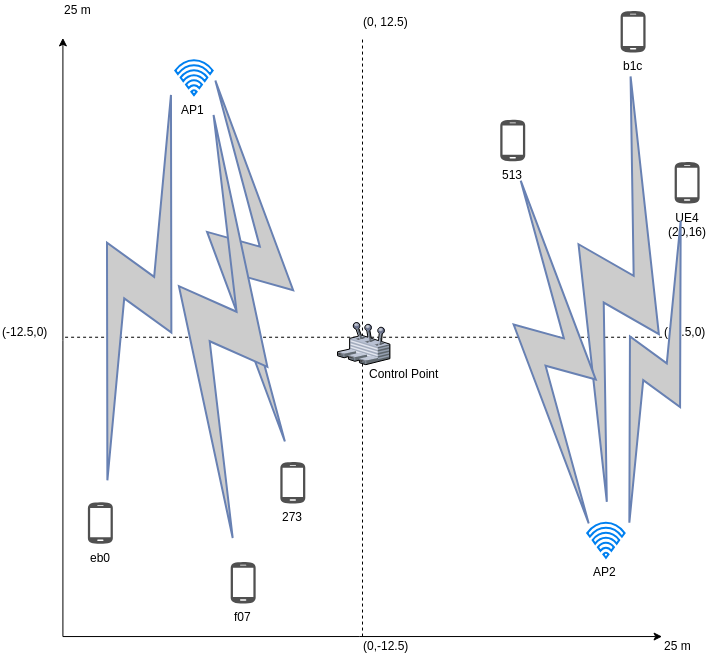
\includegraphics[width=\linewidth,keepaspectratio]{images/05-cases-description-Exp4-Near-Optimal.png}
\caption{Near-optimal layout example}
\end{figure}
